\documentclass[green]{beamer}

\usepackage[utf8]{inputenc}
\usepackage[spanish,activeacute]{babel}
\usepackage{graphicx} % Imágenes
\usepackage{fancyhdr} % Cabeceras
\usepackage{listings}

\definecolor{verde}{rgb}{0.4,0.6,0.2}
\definecolor{verdeunix}{rgb}{0.05,0.5,0.05}
\definecolor{verde2}{rgb}{0.2,0.5,0.2}

\usetheme{Berlin}
\usecolortheme[named=verdeunix]{structure}

\title{IberOgre y Sion Tower \\ V Concurso Universitario de Software Libre}
\author{David Saltares Márquez}
\date{23 de marzo de 2011}

\AtBeginSection[]
{
    \begin{frame}<beamer>
    \transdissolve
        \frametitle{Índice}
        \tableofcontents[currentsection,currentsubsection]
    \end{frame}
}

\begin{document}

\begin{frame}[fragile]
\transdissolve
    \titlepage 
	
    \begin{picture}(0,0)
        \put(10,-5){
\includegraphics[scale=0.2]{img/personaje.png}}
    \end{picture}
    
    \begin{picture}(0,0)
        \put(230,25){
\includegraphics[scale=0.06]{img/iberogre.png}}
    \end{picture}
	
    {\scriptsize
	\begin{center}
	    \begin{verbatim}
	             https://forja.rediris.es/projects/cusl5-iberogre
	    \end{verbatim}
	\end{center}
    }
    
    \begin{picture}(0,0)
        \put(135,10){
\includegraphics[scale=0.4]{img/cc-by-nc-sa.png}}
    \end{picture}
\end{frame}

\begin{frame}[fragile]
\transdissolve
    \frametitle{Índice}
    \tableofcontents
\end{frame}

\section{Introducción}

\subsection{Ogre}
\begin{frame}
\transdissolve
    \frametitle{¿Qué es Ogre?}
    
    \begin{center}
	\emph{\textbf{\huge{O}}bject Oriented \textbf{\huge{G}}raphics \textbf{\huge{R}}endering \textbf{\huge{E}}ngine}
    \end{center}
    
    Motor de renderizado 3D LGPL compatible con C++
    
    \scriptsize{
    \begin{columns}[t]
    \column{150pt}
	\begin{block}{Ofrece}
            \begin{itemize}
                \item Abstracción de OpenGL y DirectX.
		\item Gestión del grafo de escena.
                \item Modelos 3D animados, efectos de partículas, shaders, etc.
                \item Extensible y configurable.
            \end{itemize}            
        \end{block}

    \column{150pt}
	\begin{alertblock}{No ofrece}
            \begin{itemize}
                \item Colisiones.
		\item Audio.
                \item Entrada de usuario.
                \item Red.
            \end{itemize}            
        \end{alertblock}
    \end{columns} 
    }
\end{frame}

\begin{frame}
    \frametitle{Utilizado en juegos libres...}
    
    \begin{center}
	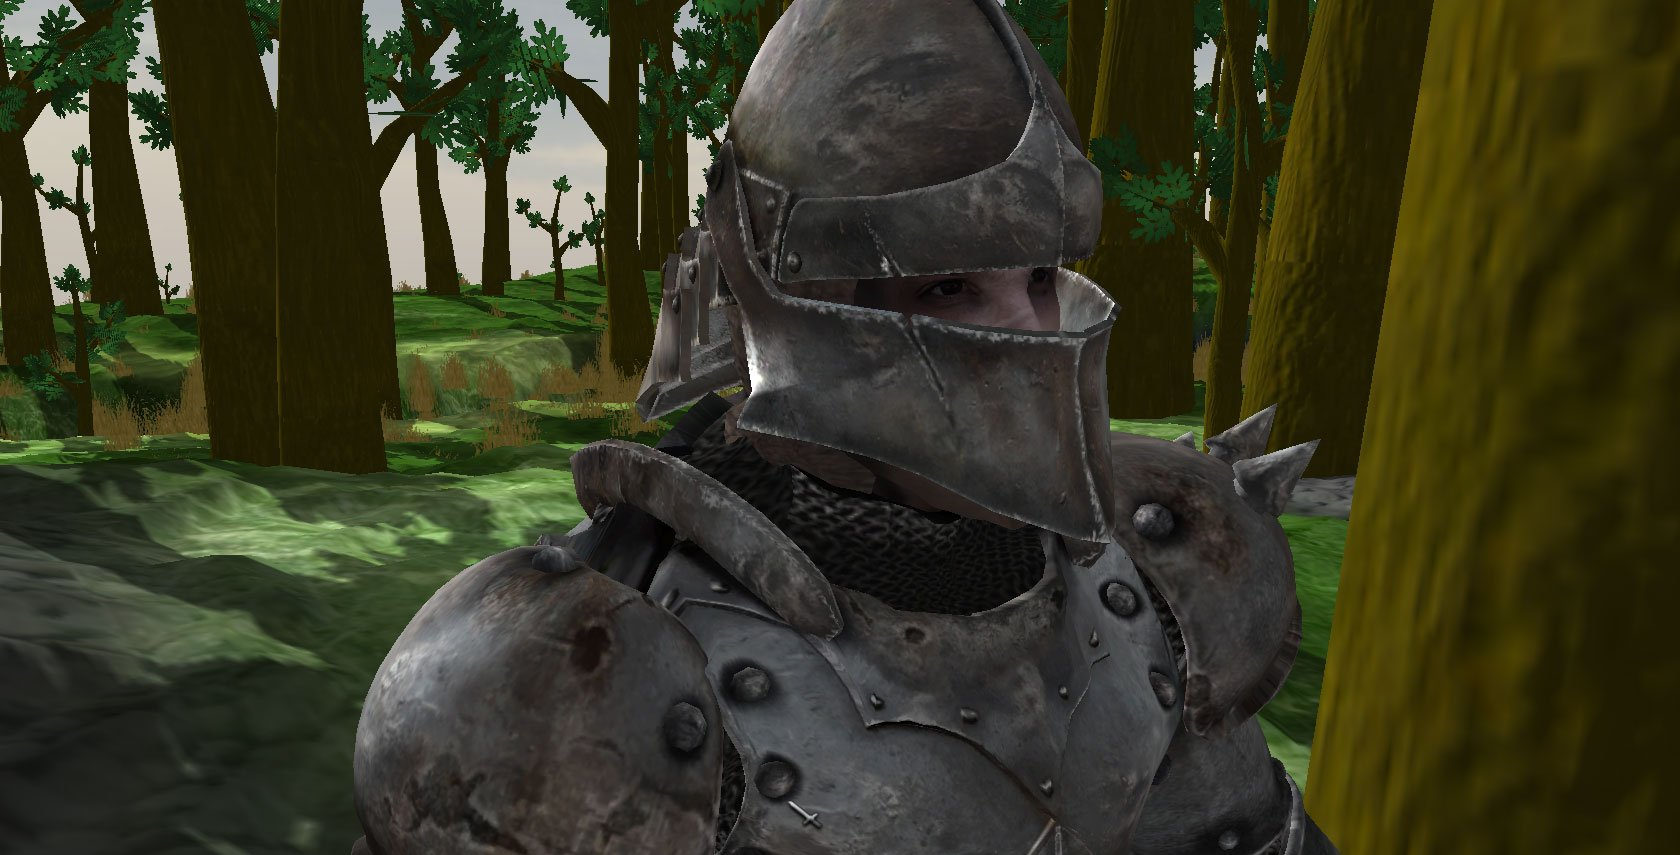
\includegraphics[scale=0.18]{img/abaddon.jpg}
	    
	\tiny{Abaddon}
    \end{center}
\end{frame}

\begin{frame}
    \frametitle{Utilizado en juegos libres...}
    
    \begin{center}
	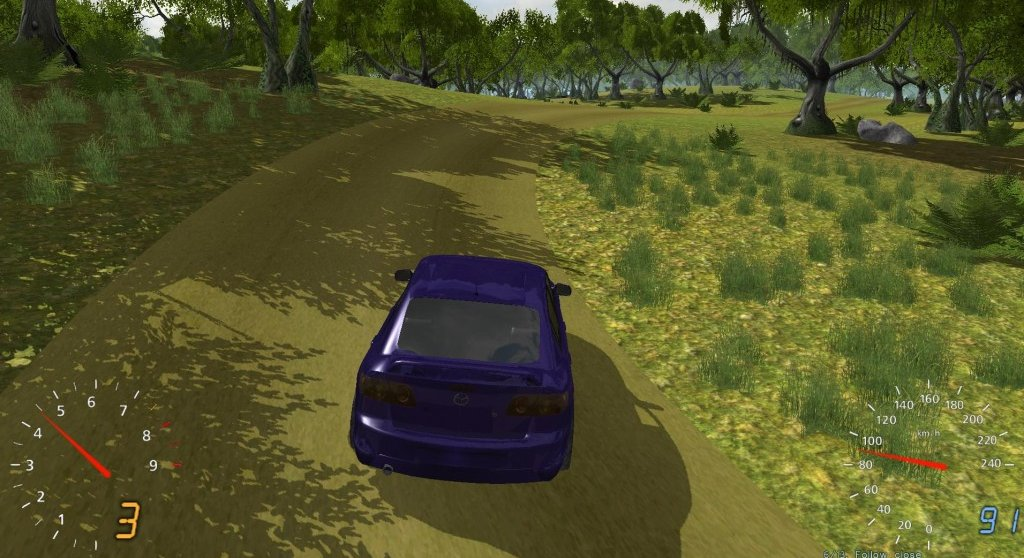
\includegraphics[scale=0.25]{img/stuntrally.jpg}
	    
	\tiny{Stunt Rally}
    \end{center}
\end{frame}

\begin{frame}
    \frametitle{... Y también en juegos comerciales}
    
    \begin{center}
	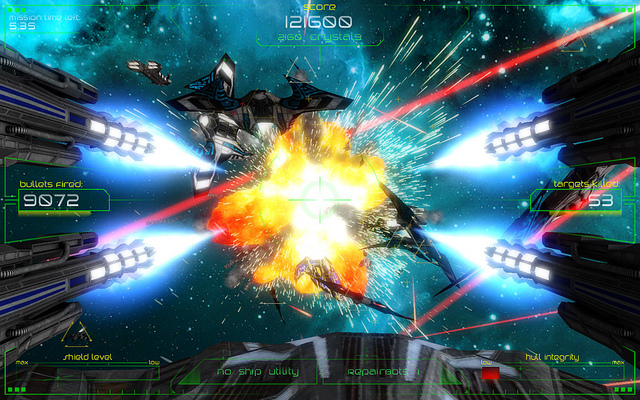
\includegraphics[scale=0.4]{img/aliendominion.jpg}
	    
	\tiny{Alien Dominion}
    \end{center}
\end{frame}

\begin{frame}
    \frametitle{... Y también en juegos comerciales}
    \begin{center}
	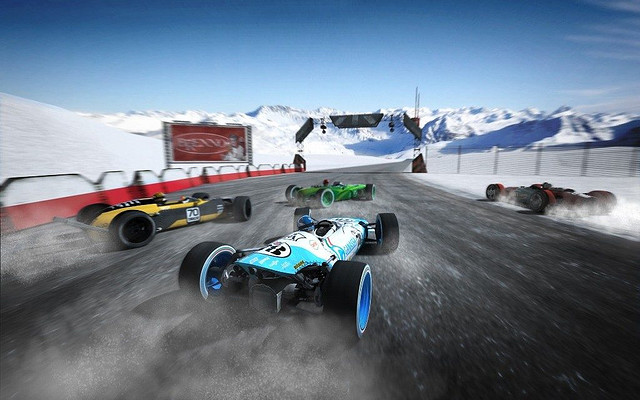
\includegraphics[scale=0.4]{img/victory.jpg}
	    
	\tiny{Victory: Age of Racing}
    \end{center}
\end{frame}

\subsection{IberOgre}

\begin{frame}
\transdissolve
    \frametitle{¿Qué es IberOgre?}
    
    Wiki en español sobre desarrollo de videojuegos en 3D con Ogre.

    \begin{columns}[c]
    \column{200pt}
        
	\begin{block}{Objetivos}
            \begin{itemize}
                \item Uso de Ogre y conocimientos matemáticos.
                \item Artículos, pequeños y grandes ejemplos.
                \item Cubrir el vacío de documentación.
                \item Apoyar el uso de software libre.
		\item Salto 2D a 3D.
            \end{itemize}            
        \end{block}

    \column{100pt}
	\begin{center}
	    
\includegraphics[scale=0.08]{img/iberogre.png}
	\end{center}
    \end{columns} 
\end{frame}

\begin{frame}
\transdissolve
	\frametitle{¿Por qué IberOgre?}
    
    \begin{columns}[c]
    \column{200pt}
        
	\begin{block}{Motivaciones}
            \begin{itemize}
                \item Cubrir vacío de documentación en castellano.
                \item Enfoque distinto a la wiki oficial.
		\item Especial atención al Software Libre.
		\item Complemento de wikijuegos (SDL).
            \end{itemize}            
        \end{block}

    \column{100pt}
	\begin{center}
	    
\includegraphics[scale=0.2]{img/question.png}
	\end{center}
    \end{columns} 
\end{frame}

\subsection{Sion Tower}

\begin{frame}
\transdissolve
    \frametitle{¿Qué es Sion Tower?}
    
    Videojuego de estrategia y acción.

    \begin{columns}[c]
    \column{200pt}
        
	\begin{block}{Características}
            \begin{itemize}
                \item Desarrollado en C++.
		\item Uso de bibliotecas libres: Ogre, OIS, SDL, etc.
                \item Ejemplo final del contenido de IberOgre.
            \end{itemize}            
        \end{block}

    \column{100pt}
        
	\begin{center}
	    
\includegraphics[scale=0.2]{img/personaje.png}
	\end{center}
    \end{columns} 
\end{frame}

\begin{frame}
\transdissolve
    \frametitle{¿Por qué Sion Tower?}
        
    \begin{columns}[c]
    \column{200pt}
        
	\begin{block}{Motivaciones}
            \begin{itemize}
                \item Deseo personal de aprender a desarrollar juegos en 3D.
		\item Ejemplo de uso real de Ogre.
		\item Documentación de subsistemas concretos.
            \end{itemize}            
        \end{block}

    \column{100pt}
        
	\begin{center}
	    
\includegraphics[scale=0.2]{img/question.png}
	\end{center}
    \end{columns} 
\end{frame}

\section{Desarrollo}

\subsection{IberOgre}

\begin{frame}
    \frametitle{Estructura de los artículos}
    
    \begin{columns}[t]
    \column{150pt}
        
	\begin{block}{Artículos}
            \begin{enumerate}
                \item Introducción
		\item Requisitos previos
		\item Contenido
		\item Ejemplo
		\item Conclusiones
            \end{enumerate}            
        \end{block}
	
    \column{150pt}
        
	\begin{center}
	    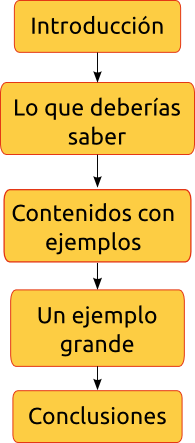
\includegraphics[scale=0.40]{img/estructura-articulos.png}
	\end{center}
	
    \end{columns} 
    
\end{frame}

\begin{frame}
\transdissolve
    \frametitle{Artículos principales (1/3)}
        
    \begin{columns}[c]
    \column{200pt}
        
	\begin{block}{Primeros pasos}
            \begin{itemize}
                \item Comenzando en IberOgre
            \end{itemize}            
        \end{block}
	
	\begin{block}{Programación de videojuegos 3D}
            \begin{itemize}
                \item Próximamente...
            \end{itemize}            
        \end{block}

    \column{100pt}
        
	\begin{center}
	    
\includegraphics[scale=0.5]{img/iberogre-cabeza.png}
	\end{center}
	
	\begin{center}
	    
\includegraphics[scale=0.25]{img/atom.png}
	\end{center}
    \end{columns} 
\end{frame}

\begin{frame}
\transdissolve
    \frametitle{Artículos principales (2/3)}
        
    \begin{columns}[c]
    \column{230pt}
        
	\scriptsize{
	\begin{block}{Ogre3D}
            \begin{itemize}
                \item Conociendo Ogre3D
		\item Conceptos Generales
		\item Instalación de Ogre3D 1.7 en GNU/Linux
		\item Instalación de Ogre3D 1.7 en Windows
		\item Creación de un entorno de trabajo multiplataforma
		\item Inicialización y cierre de Ogre
		\item Gestión de recursos
		\item Creación básica de escenas
		\item Manipulación de nodos
		\item Luces, sombras y entorno
            \end{itemize}            
        \end{block}
	}

    \column{40pt}
        
	\begin{center}
	    
\includegraphics[scale=0.3]{img/ogre.png}
	\end{center}
	
	\begin{center}
	    
\includegraphics[scale=0.3]{img/tux.png}
	\end{center}
	
	\begin{center}
	    
\includegraphics[scale=0.3]{img/trabajo.png}
	\end{center}
	
	\begin{center}
	    
\includegraphics[scale=0.3]{img/pintura.png}
	\end{center}
	
	\begin{center}
	    
\includegraphics[scale=0.3]{img/arbol.png}
	\end{center}
	
	\column{40pt}
	
	\begin{center}
	    
\includegraphics[scale=0.3]{img/castillo.png}
	\end{center}
	
	\begin{center}
	    
\includegraphics[scale=0.3]{img/windows.png}
	\end{center}
	
	\begin{center}
	    
\includegraphics[scale=0.3]{img/engranaje.png}
	\end{center}
	
	\begin{center}
	    
\includegraphics[scale=0.3]{img/claqueta.png}
	\end{center}
	
	\begin{center}
	    
\includegraphics[scale=0.3]{img/entorno.png}
	\end{center}
	
    \end{columns} 
\end{frame}

\begin{frame}
\transdissolve
    \frametitle{Artículos principales (3/3)}
        
    \begin{columns}[c]
    \column{200pt}
        
	\begin{block}{Otras tecnologías}
            \begin{itemize}
                \item Manejo básico de OIS
		\item Exportar modelos desde Blender
            \end{itemize}            
        \end{block}

    \column{100pt}
        
	\begin{center}
	    
\includegraphics[scale=0.5]{img/joystick.png}
	\end{center}
	
	\begin{center}
	    
\includegraphics[scale=0.5]{img/blender-icono.png}
	\end{center}
    \end{columns} 
\end{frame}

\begin{frame}
\transdissolve
    \frametitle{Estadísticas}

    \begin{columns}[t]
    \column{150pt}
        
	\begin{block}{Haciendo números}
            \begin{itemize}
                \item \textbf{Páginas}: 131
		\item \textbf{Ediciones}: 441
		\item \textbf{Usuarios}: 11
		\item \textbf{Visitas}: 9.255
            \end{itemize}            
        \end{block}

    \column{150pt}

	\begin{center}
	    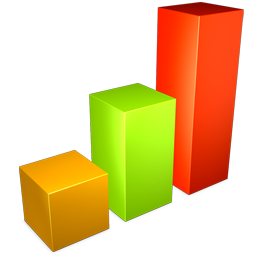
\includegraphics[scale=0.25]{img/estadisticas.png}
	\end{center}

    \end{columns} 

\end{frame}

\subsection{Sion Tower}

% GDD
\begin{frame}
\transdissolve
    \frametitle{Documento de diseño}
    
    \begin{center}
	
\includegraphics[scale=0.4]{img/libro.png}
    \end{center}
    
    \scriptsize{
    \begin{columns}[t]
    \column{150pt}
        
	\begin{block}{Contiene}
            \begin{itemize}
                \item Descripción del juego.
		\item Mecánicas.
		\item Personajes, objetos y habilidades.
		\item Interfaz.
		\item Lista de recursos.
            \end{itemize}            
        \end{block}

    \column{150pt}
        
	\begin{block}{Me ayudó a}
            \begin{itemize}
                \item Dejar por escrito lo que iba a desarrollar.
		\item Conseguir colaboradores.
		\item Misma concepción del juego.
            \end{itemize}            
        \end{block}
    \end{columns} 
    }
\end{frame}

% Sonido 3D
\begin{frame}
\transdissolve
    \frametitle{Audio 3D}
    
    \tiny{
    \begin{center}
	Liberado en un paquete independiente.
    \end{center}
    }
    
    \begin{columns}[c]
    \column{150pt}
        
	\scriptsize{
	\begin{block}{Características}
            \begin{itemize}
                \item Sonidos adjuntos a nodos de la escena (emisor).
		\item Un nodo hace de escucha.
		\item Variación de volumen y efecto estéreo.
		\item Integrado con la gestión de recursos de Ogre.
            \end{itemize}            
        \end{block}
	}
	
	

    \column{150pt}
        
	\begin{center}
	    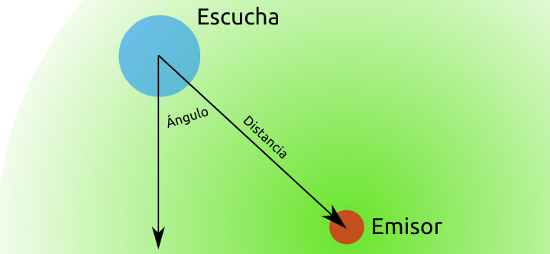
\includegraphics[scale=0.9]{img/audio3d-esquema.png}
	\end{center}
	
    \end{columns} 
\end{frame}


% Colisiones
\begin{frame}
\transdissolve
    \frametitle{Detección de colisiones}
    
    \tiny{
    \begin{center}
	Liberado en un paquete independiente.
    \end{center}
    }
    
    
    \begin{columns}[t]
    \column{150pt}
        
	\tiny{
	\begin{block}{Características}
            \begin{itemize}
                \item \textbf{Shapes}: esfera, plano, AABB y OBB.
		\item \textbf{Body}: conjunto de Shapes.
		\item \textbf{GameObject}: Body (colisionable) + Entity (visual).
		\item \textbf{Colisiones}: a nivel de Shape o Body.
		\item \textbf{Callbacks}: al comienzo, durante y al finalizar colisión.
		\item \textbf{Filtrado}: colisiones entre ciertos tipos de Body.
            \end{itemize}            
        \end{block}
	}
	
	\begin{center}
	    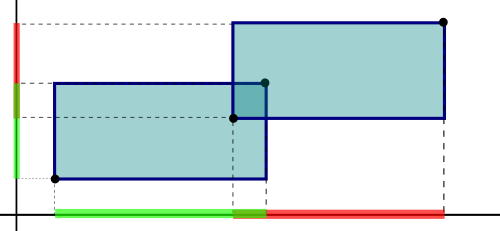
\includegraphics[scale=0.3]{img/test-aabb-aabb.png}
	\end{center}

    \column{150pt}
	
	\begin{center}
	    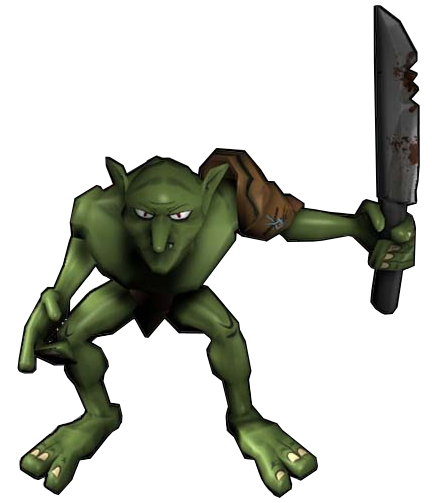
\includegraphics[scale=0.3]{img/goblin.png}
	\end{center}
	
    \end{columns} 
\end{frame}

% Carga de escenarios desde Blender
\begin{frame}
\transdissolve
    \frametitle{Carga de escenarios desde Blender}
    
    \begin{columns}[t]
    \column{150pt}
        
	\scriptsize{
	\begin{block}{Características}
            \begin{itemize}
                \item Creación y posicionamiento de objetos.
		\item Exportación a formato \emph{DotScene} (xml).
		\item Carga del escenario en el sistema.
		\item Fácil de modificar.
		\item Información extra: posición de comienzo, navegación, etc.
		\item ¡No hay que recompilar!
            \end{itemize}            
        \end{block}
	}

    \column{150pt}
	
	\begin{center}
	    
\includegraphics[scale=0.5]{img/blender-icono.png}
	\end{center}
	
	\begin{center}
	    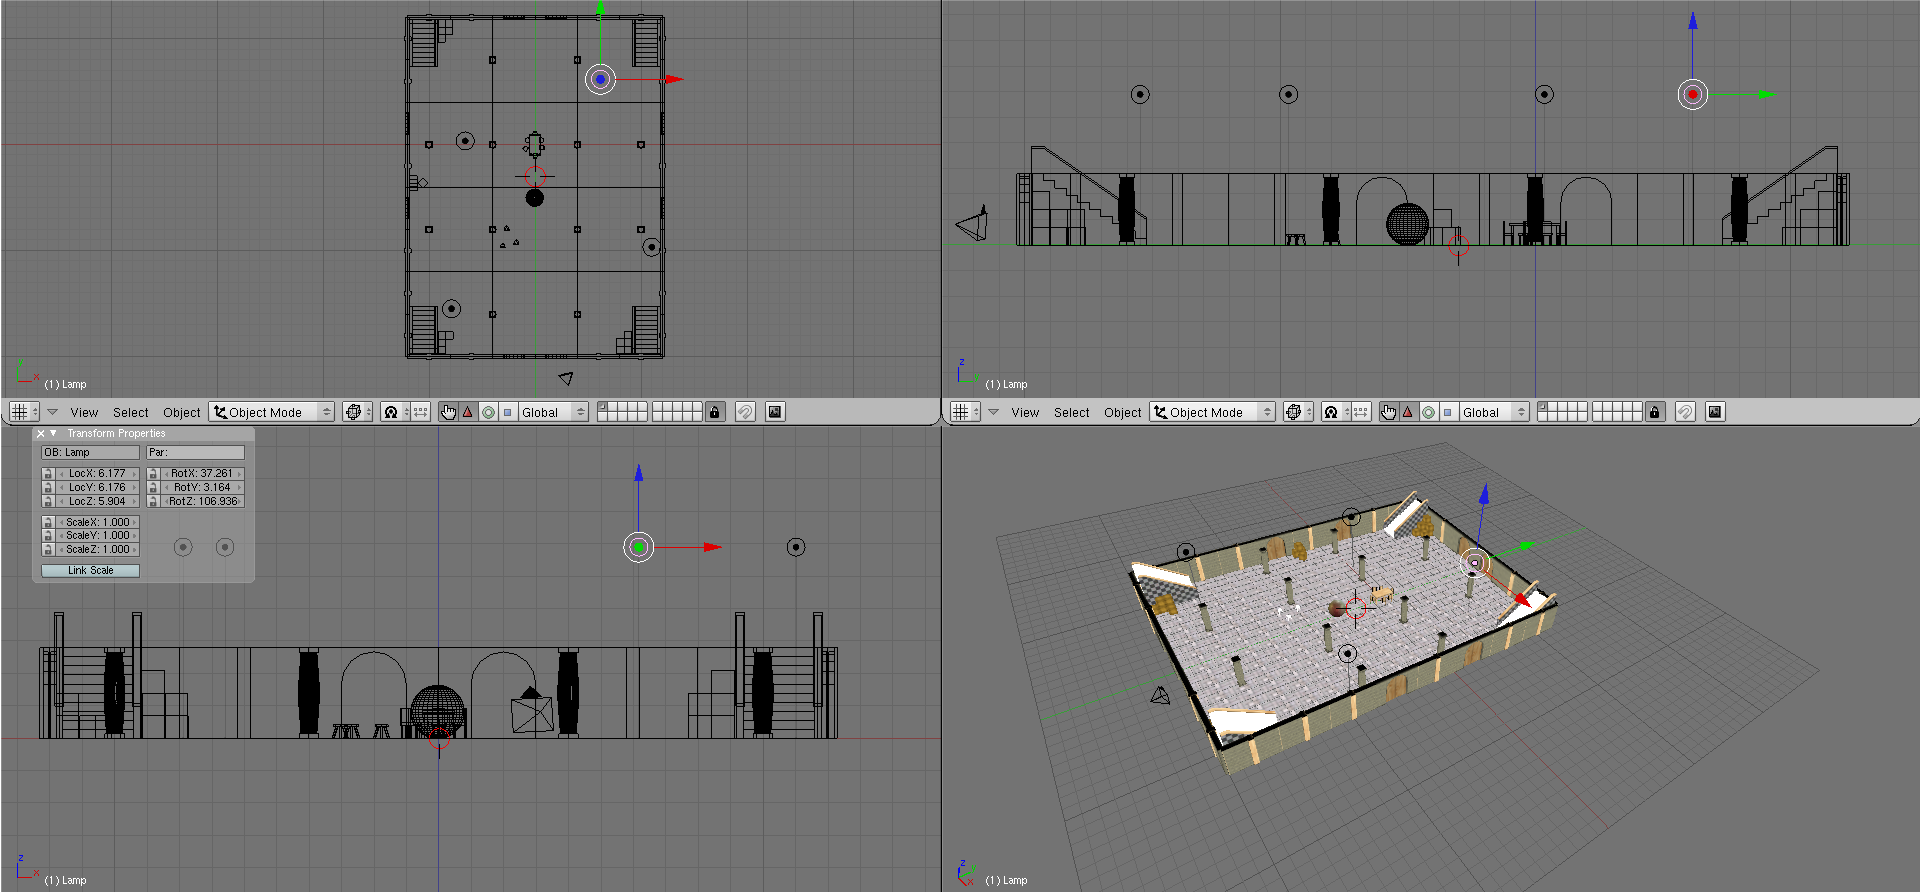
\includegraphics[scale=0.08]{img/escenarios-blender.png}
	\end{center}
	
    \end{columns} 
\end{frame}

\section{Comunidad}

\subsection{Colaboraciones}

% Alberto Cejas Sánchez: Artículo arquitectura
% Mario Velázquez Muñoz: Manual Ogre3D
% Antonio Jiménez Rodríguez (AJR): arte 3D
% Estudio Evergreen (Antonio Caro Oca y Daniel Pellicer): BSO

\begin{frame}
\transdissolve
    \frametitle{Colaboraciones}
    
    \begin{center}
	
\includegraphics[scale=0.10]{img/colaboradores.jpg}
    \end{center}
    
    \begin{columns}[t]
    \column{150pt}
        
	\scriptsize{
	\begin{block}{Colaboradores}
            \begin{itemize}
                \item Alberto Cejas Sánchez: artículo \emph{Conceptos generales}
		\item Mario Velázquez Muñoz: manual Ogre3D en español.
		\item Antonio Jiménez Rodríguez: arte 3D.
		\item Estudio Evergreen (Antonio Caro Oca y Daniel Pellicer): BSO
		\item Ediciones en IberOgre.
            \end{itemize}            
        \end{block}
	}

    \column{150pt}
	
	\begin{center}
	    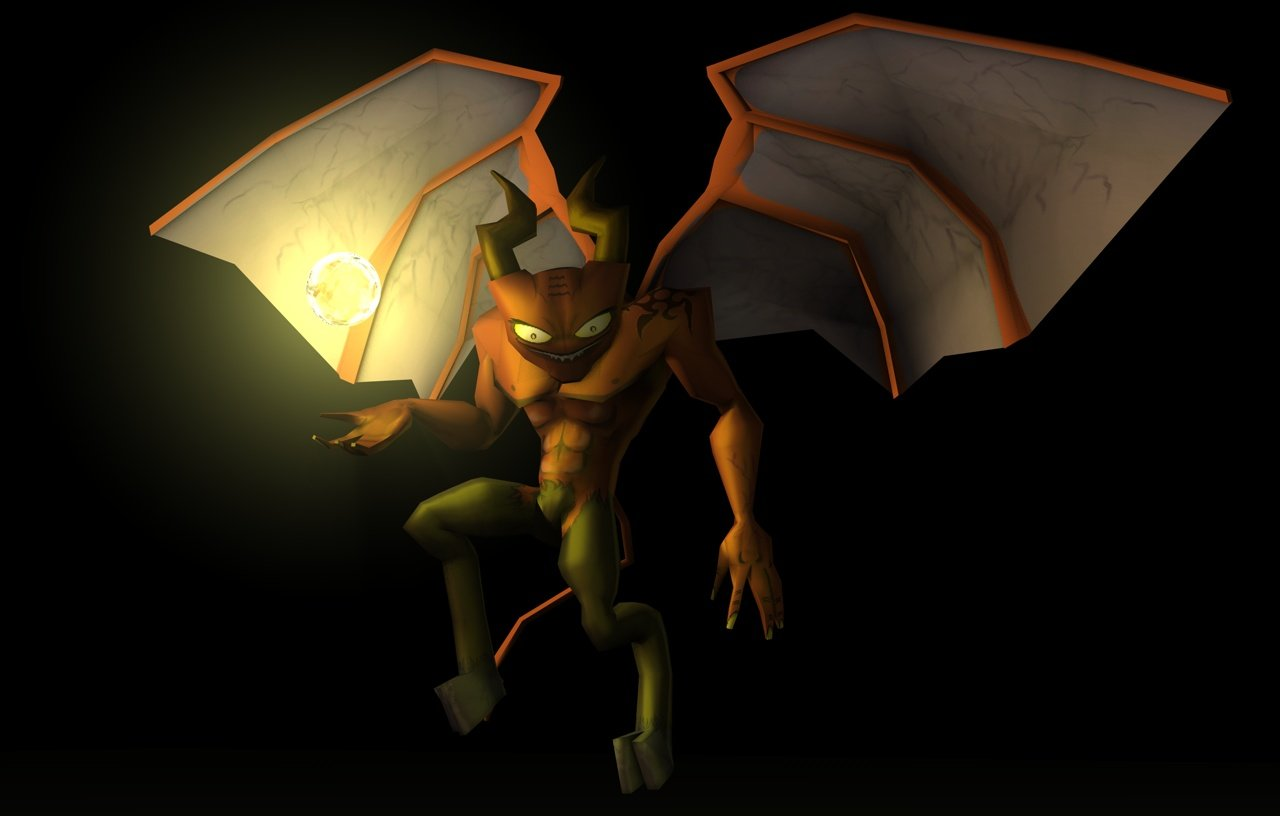
\includegraphics[scale=0.11]{img/diablillo.jpg}
	\end{center}
	
    \end{columns} 
\end{frame}

\subsection{Difusión}

% Twitter (opinión y Steve Streeting)
% Blog artículos
% Visitas al blog 
% Visitas a IberOgre
% Web oficial de Ogre3D
\begin{frame}
\transdissolve
    \frametitle{Difusión}
    
    \begin{columns}[t]
    \column{200pt}
	
	\scriptsize{
	\begin{block}{Medios}
            \begin{itemize}
                \item \textbf{Twitter}: 63 seguidores con muchas sugerencias y opiniones.
		\item \textbf{Blog}: 57 artículos y 43.761 visitas.
		\item \textbf{Forja}: entre los proyectos más activos.
		\item \textbf{Apariciones}: web oficial de Ogre y varias comunidades hispano-hablantes.
            \end{itemize}            
        \end{block}
	
	\begin{block}{}
            http://twitter.com/IberOgre
	    http://siondream.com/blog/category/proyectos/pfc
	    https://forja.rediris.es/projects/cusl5-iberogre
        \end{block}
	}
	

    \column{100pt}
	
    \begin{center}
	    
\includegraphics[scale=0.25]{img/twitter.png}
    \end{center}
    \begin{center}
	    
\includegraphics[scale=0.13]{img/blog.png}
    \end{center}
    \begin{center}
	    
\includegraphics[scale=0.5]{img/rediris.png}
    \end{center}
	
    \end{columns} 
\end{frame}

\section{Demostración}

\begin{frame}
\transdissolve
    \frametitle{Demostración}
    
    \begin{center}
	Veamos IberOgre y Sion Tower en directo
    \end{center}
    
    
    \begin{columns}[c]
    \column{175pt}
        
	\begin{center}
	    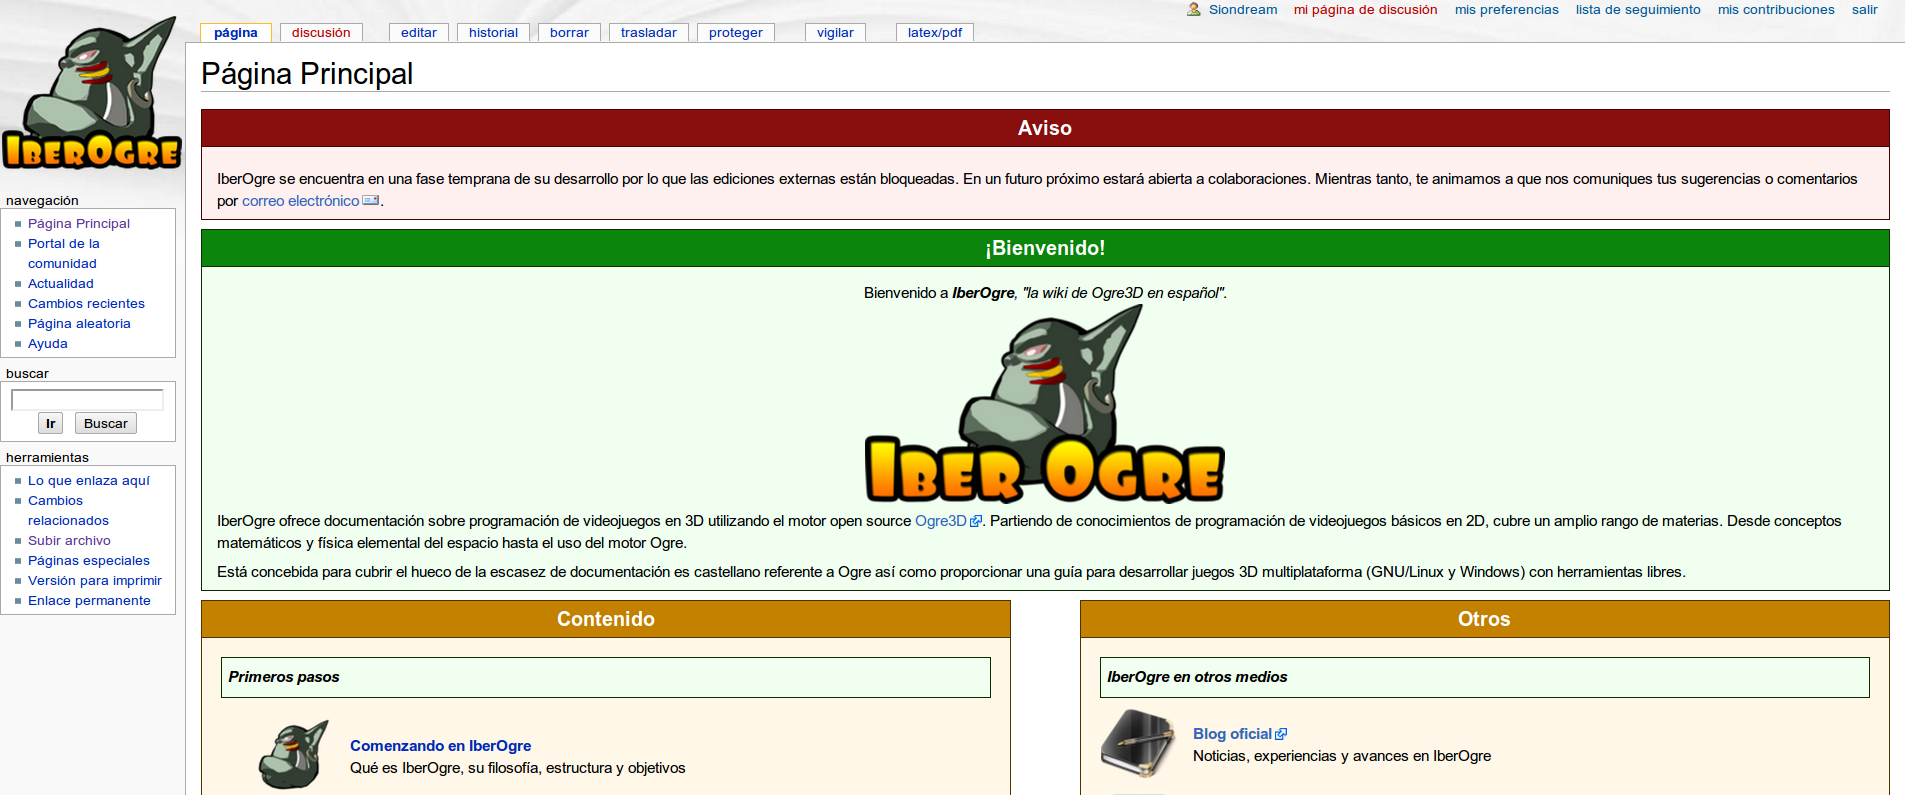
\includegraphics[scale=0.09]{img/captura-iberogre.png}
	\end{center}

    \column{175pt}
        
	\begin{center}
	    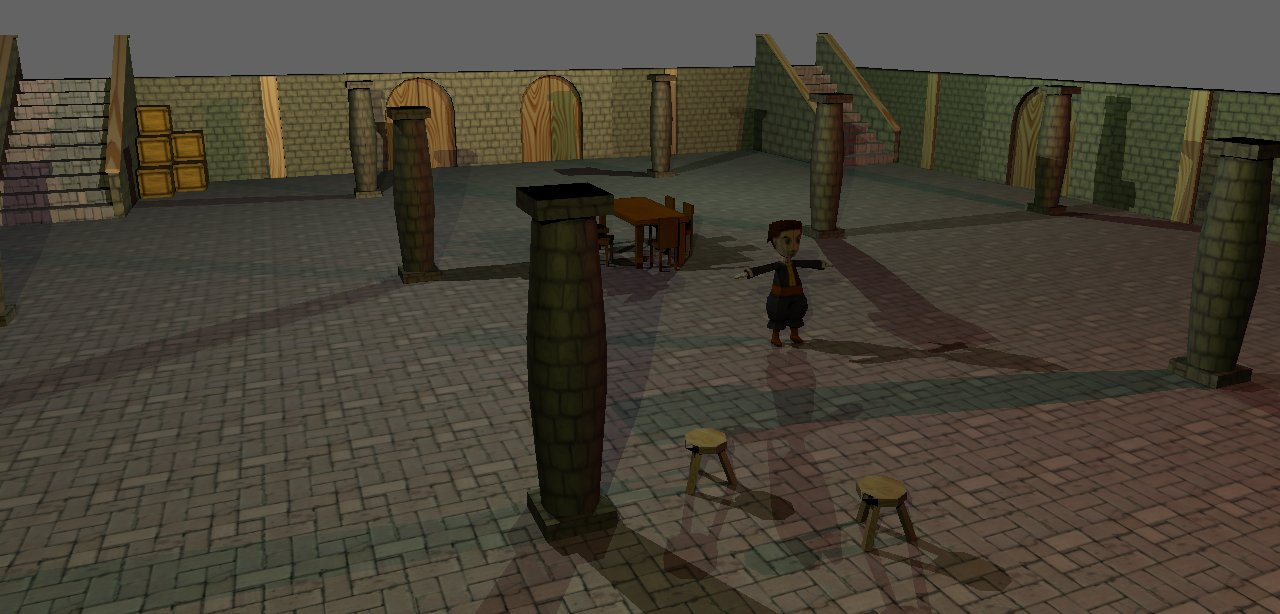
\includegraphics[scale=0.1]{img/captura-siontower.jpg}
	\end{center}
    \end{columns} 
\end{frame}

\begin{frame}
\transdissolve
    \frametitle{}
    
    \begin{center}
	\huge{\textbf{¡Muchas gracias!}}
    \end{center}
    
    \begin{center}
	\textbf{¿Preguntas?}
    \end{center}
    
    \begin{center}
	    
\includegraphics[scale=0.25]{img/pregunta.png}
    \end{center}
    
\end{frame}


\end{document}
